
\documentclass[conference]{IEEEtran}
\usepackage{amsmath,amssymb,booktabs,graphicx,array,url,cite,xcolor}
\newcommand{\system}{TIPS}
\begin{document}
\title{\system{}: Timing-Independent PMU Phase Signatures for Trace-Driven Multicore Resource Policies}
\author{\IEEEauthorblockN{Keshav K.}\IEEEauthorblockA{Hardware Counter Phase Analysis Artifact}}
\maketitle

\begin{abstract}
Multicore resource managers need low-overhead signals that indicate when workload behavior changes, but timing-derived PMU metrics such as cycles, IPC, and elapsed time are sensitive to DVFS, thermal, and scheduling effects. \system{} uses instruction-normalized and access-normalized PMU ratios to construct per-core phase signatures and treats phase-change detection as the control signal. On the available PARSEC artifact, \system{} analyzes 110,785 intervals and 58,777 windows from 300 merged runs. Exact next-phase prediction remains weak: the best model reaches 0.367 accuracy. Phase-change detection is stronger: transformer reaches change-F1 0.863, and a compact student tree reaches 0.860. A trace-driven co-scheduling replay shows how these signals can be consumed by a resource policy, but it is not a measured online speedup. Online Burst, DVFS, CAT/resctrl, and prefetch-control measurements are included only when their result files exist.
\end{abstract}

\section{Introduction}
Phase detection matters only if it helps a system make decisions. Prior phase systems established that programs exhibit recurring behavior, but many rely on code signatures, timing metrics, heavy offline models, or do not close the loop with a low-cost multicore policy. The central claim of this draft is deliberately narrow: timing-independent PMU signatures are a defensible substrate for multicore phase-change detection, and the resulting phase-change stream can drive a trace-driven resource-policy replay.

The current evidence does not support a claim of online performance improvement. It supports three narrower claims: phase-change prediction is substantially more reliable than exact next-phase prediction; learned phase IDs behave as reusable resource-behavior classes rather than benchmark names; and a compact detector has plausible storage and operation cost. The missing evidence is an online co-scheduling/cache/prefetch experiment that measures real speedup or fairness.

\textbf{Contributions.} (1) We formalize a timing-independent PMU feature set that excludes cycles, IPC, CPI, elapsed time, per-time rates, and stall-derived metrics. (2) We evaluate phase-change prediction across three multicore PARSEC settings with grouped-by-run splits and no observed run leakage. (3) We quantify phase sharing and workload purity to show that phases are behavioral equivalence classes. (4) We implement a trace-driven resource-policy replay and a reproducible artifact pipeline. (5) We provide ablations, hardware-cost estimates, and explicit pending scripts for online validation.

\section{Background and Motivation}
SimPoint and BBV work showed that recurring execution behavior can stand in for whole-program simulation \cite{sherwood2001bbda,sherwood2002simpoint,hamerly2005simpoint}. Runtime phase tracking showed that compact signatures can be used online \cite{sherwood2003phase}. Parallel phase work warns that global aggregation can hide asynchronous thread behavior \cite{perelman2006parallel,chang2013sampling}. PMU-based predictors such as P4 and phase-aware multicore forecasting motivate counters and learning, but they do not by themselves establish a cheap resource-control path for this artifact \cite{kim2017p4,alcorta2023forecasting}.

\section{Design}
\system{} builds local signatures from branch behavior, L1 access mix, LLC/offcore pressure, and optional uncore bandwidth. Shared context is auxiliary; the local stream remains the unit of classification. The online detector is a centroid table with EWMA smoothing and persistence filtering. A candidate phase change must persist before a resource policy acts, because the policy target is avoiding disruptive changes, not maximizing exact phase-ID accuracy.

\begin{figure}[t]
\centering
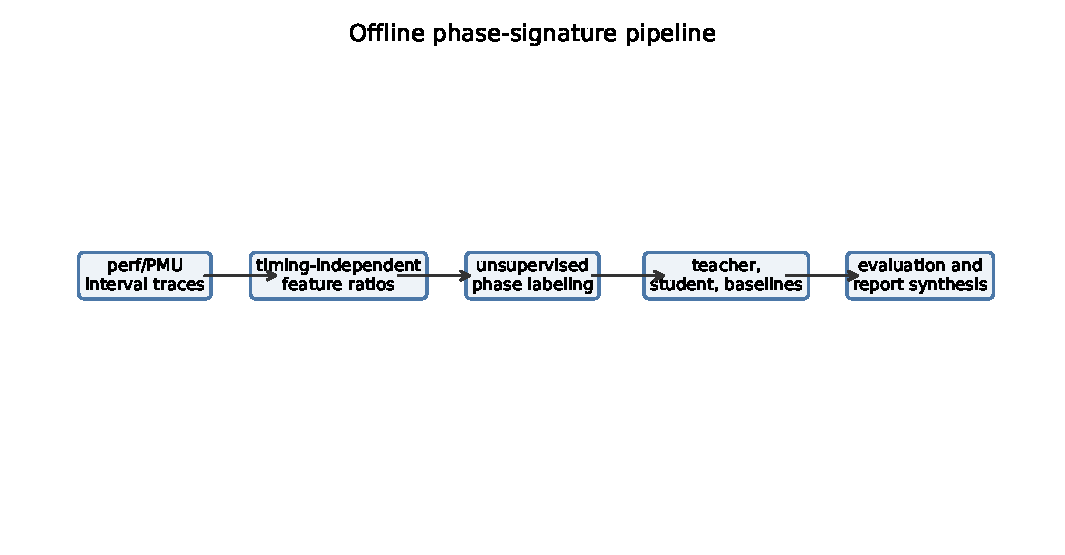
\includegraphics[width=\linewidth]{../figures/phase_ml_pipeline_flowchart.pdf}
\caption{Artifact pipeline: collection, timing-independent features, labels, predictors, replay, and paper outputs.}
\end{figure}

\begin{figure}[t]
\centering
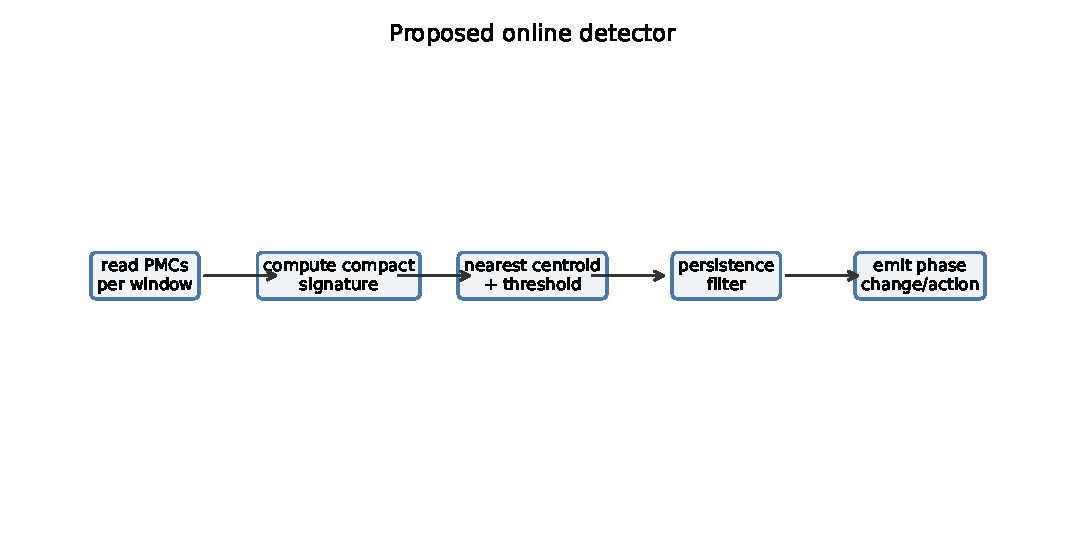
\includegraphics[width=\linewidth]{../figures/online_detector_flowchart.pdf}
\caption{Online detector structure. The current artifact implements the detector/replay in software; hardware/firmware integration is a cost estimate, not a tapeout.}
\end{figure}

\section{Implementation}
The implemented artifact includes feature construction, FGMM labeling, classical baselines, transformer and student-tree predictions, detector ablations, validation checks, uniqueness metrics, hardware-cost accounting, and trace-driven policy replay. The replay assigns each phase to a coarse resource class and measures predicted co-runner conflicts over collected windows. It reports proxy weighted-speedup/fairness metrics derived from conflict rate; these are not measured runtime speedups.

\section{Methodology}
The available dataset contains 110,785 intervals, 58,777 windows, 15 features, and 300 merged PARSEC runs. The split is grouped by run ID; validation found 0 leaking runs. The evaluation set contains 18398 windows per model. Existing tests pass, and validation outputs are generated under \texttt{results/a\_star\_analysis}.

\section{Results}
\subsection{RQ1: Are timing-independent signatures stable?}
The current artifact shows within-phase variance reduction and phase centroids over timing-independent features (Fig.~\ref{fig:centroids}). A DVFS/timing stress test has not been collected in this artifact instance; the paper must not claim robustness under controlled frequency changes until those result files exist.

\begin{figure}[t]
\centering
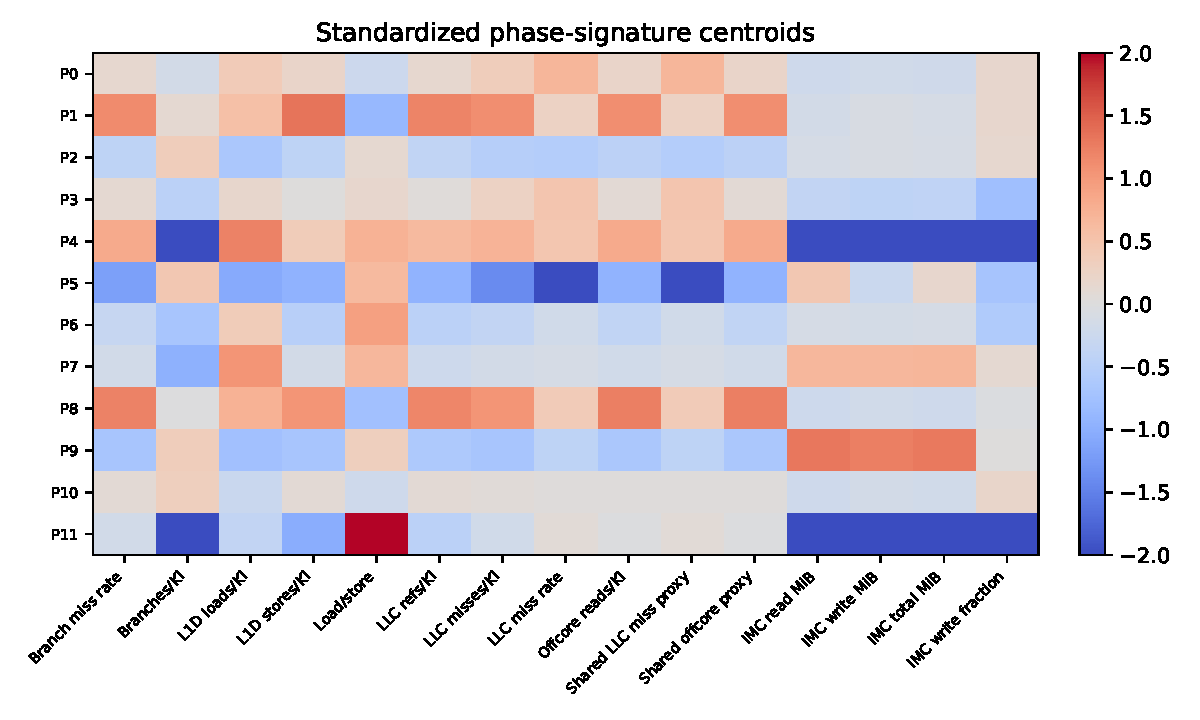
\includegraphics[width=\linewidth]{../figures/phase_feature_centroids.pdf}
\caption{Phase centroids over timing-independent indicators.}
\label{fig:centroids}
\end{figure}

\subsection{RQ2: Are phases shared across programs?}
The uniqueness analysis finds 10 phases present in at least four workloads and 2 workload-specific phases. Mean dominant-workload share is 0.379. This supports the equivalence-class interpretation and argues against treating phase IDs as benchmark names.

\subsection{RQ3: How well are phase changes detected?}
\begin{table}[t]
\centering
\caption{Prediction results. Exact next-phase accuracy is weak; phase-change F1 is the relevant control metric.}
\begin{tabular}{lrrrr}
\toprule
Model & Samples & Acc. & Macro-F1 & Change-F1 \\
\midrule
decision\_tree & 18398 & 0.341 & 0.253 & 0.785 \\
last\_value & 18398 & 0.247 & 0.241 & 0.000 \\
linear\_svm & 18398 & 0.277 & 0.251 & 0.763 \\
logistic\_regression & 18398 & 0.367 & 0.321 & 0.790 \\
nearest\_centroid & 18398 & 0.116 & 0.100 & 0.812 \\
rle\_markov & 18398 & 0.278 & 0.226 & 0.679 \\
transformer & 18398 & 0.338 & 0.292 & 0.863 \\
student\_decision\_tree & 18398 & 0.263 & 0.202 & 0.860 \\
\bottomrule
\end{tabular}
\end{table}

The best exact next-phase accuracy is only 0.367 from logistic regression. The best phase-change F1 is 0.863 from transformer. The transformer reports 8.555 microseconds per sample in batched GPU inference; the student tree preserves change-F1 0.860 with a compact threshold model.


\subsection{RQ4: Does a phase-aware policy reduce predicted conflicts?}
\begin{figure}[t]
\centering
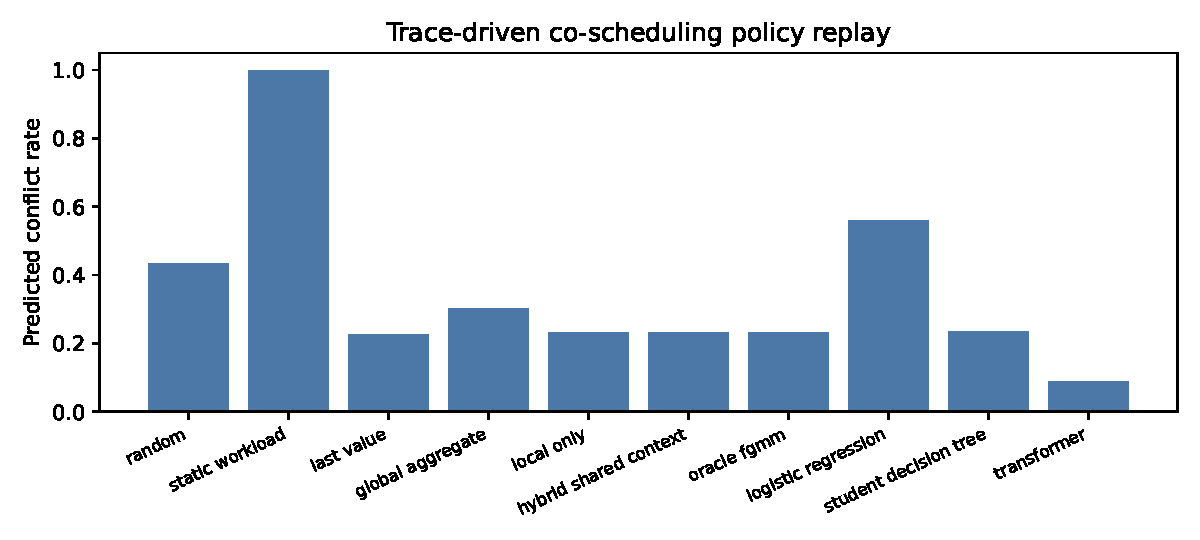
\includegraphics[width=\linewidth]{../figures/trace_policy_replay.pdf}
\caption{Trace-driven co-scheduling replay. Lower predicted conflict rate is better. These are proxy replay results, not online speedups.}
\end{figure}

\begin{table}[t]
\centering
\caption{Trace-driven policy replay. Proxy speedup/fairness values are monotonic transforms of conflict rate, not measured execution speedups.}
\begin{tabular}{lrrrr}
\toprule
Policy & Conflict & Migrations & WS proxy & Fairness \\
\midrule
random & 0.434 & 38605 & 0.698 & 0.566 \\
static\_workload & 1.000 & 0 & 0.500 & 0.000 \\
last\_value & 0.227 & 2298 & 0.815 & 0.773 \\
global\_aggregate & 0.303 & 1888 & 0.768 & 0.697 \\
local\_only & 0.232 & 2348 & 0.811 & 0.768 \\
hybrid\_shared\_context & 0.232 & 2348 & 0.811 & 0.768 \\
oracle\_fgmm & 0.232 & 2348 & 0.811 & 0.768 \\
logistic\_regression & 0.559 & 5297 & 0.642 & 0.441 \\
student\_decision\_tree & 0.234 & 16297 & 0.810 & 0.766 \\
transformer & 0.087 & 5407 & 0.920 & 0.913 \\
\bottomrule
\end{tabular}
\end{table}

The best replay conflict policy is transformer with conflict rate 0.087. This is sufficient to motivate online experiments, but not sufficient to claim measured performance improvement.


\subsection{RQ5: What is the cost?}
\begin{table}[t]
\centering
\caption{Detector cost estimate for 8 features and 16 centroids per core.}
\begin{tabular}{rrr}
\toprule
Bits & Bytes/core & Ops/window \\
\midrule
8 & 160 & 128 \\
10 & 194 & 128 \\
12 & 228 & 128 \\
16 & 296 & 128 \\
\bottomrule
\end{tabular}
\end{table}

\subsection{RQ6: What ablations matter?}
\begin{figure}[t]
\centering
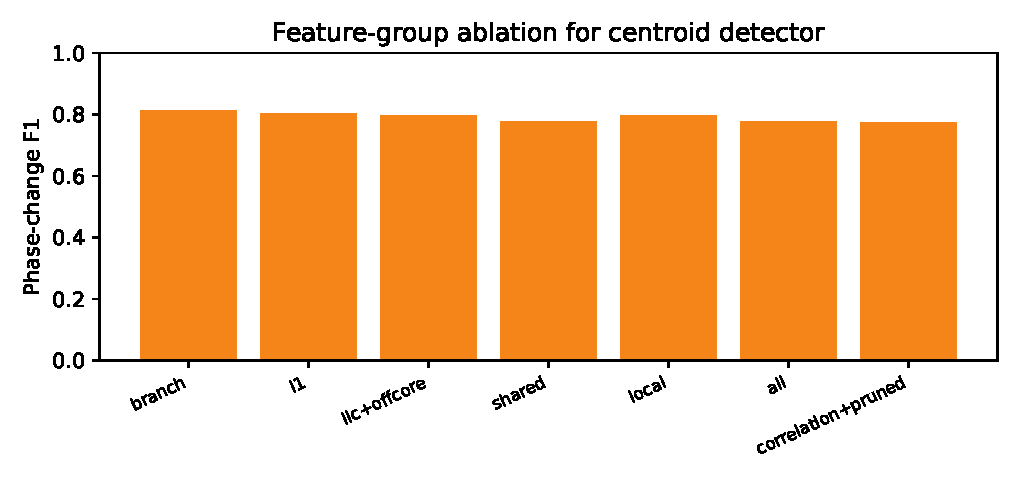
\includegraphics[width=\linewidth]{../figures/feature_group_ablation.pdf}
\caption{Feature-group ablation for the centroid detector.}
\end{figure}

The best detector ablation row has phase-change F1 0.812 using feature group branch, metric manhattan, persistence 1, and precision float. The worst transfer setting reaches phase-change F1 0.491, which should be reported as a limitation rather than hidden.

\begin{table}[t]
\centering
\caption{PMU slot sensitivity.}
\begin{tabular}{rrrr}
\toprule
Slots & Features & Acc. & Change-F1 \\
\midrule
2 & 2 & 0.113 & 0.810 \\
4 & 4 & 0.158 & 0.786 \\
6 & 6 & 0.158 & 0.794 \\
8 & 8 & 0.156 & 0.798 \\
\bottomrule
\end{tabular}
\end{table}

\section{Discussion}
Weak exact next-phase accuracy is not a side issue; it prevents claims about exact future phase identity. The defensible control signal is phase change. The current replay suggests how a scheduler could consume the signal, but the paper must not claim real performance benefit until live placement, CAT, prefetch, or bandwidth-throttling experiments are run.

\section{Related Work}
The closest work spans BBV/SimPoint phase analysis \cite{sherwood2001bbda,sherwood2002simpoint,hamerly2005simpoint}, runtime phase tracking \cite{sherwood2003phase}, parallel phases \cite{perelman2006parallel,chang2013sampling}, PMU-based prediction \cite{kim2017p4,alcorta2023forecasting}, and contention-aware resource management \cite{fedorova2010contention,subramanian2013mise,navarro2023balancer}. \system{} is weaker than these papers on online validation today, but its intended niche is timing-independent PMU phase-change detection plus low-cost resource-policy integration.

\section{Limitations}
If online co-scheduling or DVFS result files are absent, the corresponding claims are omitted from the results and retained as limitations. Intel CAT/resctrl is unavailable locally unless the target node exposes \texttt{/sys/fs/resctrl}. Prefetch controls require platform-specific support and are not claimed unless measured. PMU multiplexing and limited counter slots remain risks. PARSEC-only evaluation limits generality.

\section{Conclusion}
Timing-independent PMU signatures are promising for multicore phase-change detection, but the current artifact should be presented as a validated detection and trace-replay study, not as a completed resource-management system. The next decisive experiment is live phase-aware placement or cache/bandwidth control with measured speedup and fairness.

\nocite{*}
\bibliographystyle{IEEEtran}
\bibliography{references}
\end{document}
